\newpage
\chapter*{\centering{\MakeUppercase{2. NHẬP MÔN PYTHON}}}
\addcontentsline{toc}{chapter}{\textcolor{fitblue}{\MakeUppercase{2. NHẬP MÔN PYTHON}}}

\noindent \indent Mặc dù mỗi ngôn ngữ lập trình đều khác nhau (tuy không khác biệt nhiều như các nhà thiết kế ngôn ngữ muốn chúng ta tin tưởng), vẫn có một số tiêu chí để liên kết chúng lại với nhau:

\begin{itemize}
    \item \textbf{Bậc thấp so với bậc cao (Low-level versus high-level):} Đề cập đến việc chúng ta lập trình bằng các chỉ lệnh và đối tượng dữ liệu ở cấp độ máy (ví dụ: di chuyển 64 bit dữ liệu từ vị trí này sang vị trí khác) hay lập trình bằng các thao tác trừu tượng hơn (ví dụ: làm xuất hiện một menu trên màn hình) do nhà thiết kế ngôn ngữ cung cấp.

    \item \textbf{Đa năng so với Chuyên biệt (General versus targeted to an application domain):} Đề cập đến việc các thao tác sơ khai của ngôn ngữ lập trình có khả năng ứng dụng rộng rãi hay được tinh chỉnh cho một miền cụ thể. Ví dụ, SQL được thiết kế để tạo thuận lợi cho việc trích xuất thông tin từ các cơ sở dữ liệu quan hệ, nhưng bạn sẽ không muốn sử dụng nó để xây dựng một hệ điều hành.

    \item \textbf{Thông dịch so với Biên dịch (Interpreted versus compiled):} Đề cập đến việc chuỗi các chỉ lệnh do lập trình viên viết, gọi là mã nguồn (source code), được thực thi trực tiếp (bởi một trình thông dịch) hay trước tiên nó được chuyển đổi (bởi một trình biên dịch) thành một chuỗi các thao tác sơ khai cấp độ máy. (Vào thời kỳ đầu của máy tính, con người phải viết mã nguồn bằng một ngôn ngữ rất gần với mã máy để có thể được phần cứng máy tính thông dịch trực tiếp). Cả hai phương pháp đều có ưu điểm. Thông thường, việc gỡ lỗi (debug) các chương trình viết bằng ngôn ngữ thông dịch sẽ dễ dàng hơn, vì trình thông dịch có thể tạo ra các thông báo lỗi dễ dàng đối chiếu với mã nguồn. Các ngôn ngữ biên dịch thường tạo ra các chương trình chạy nhanh hơn và tốn ít không gian lưu trữ hơn.
\end{itemize}

Trong cuốn sách này, chúng ta sử dụng Python. Tuy nhiên, cuốn sách này không phải nói về Python. Nó chắc chắn sẽ giúp người đọc học Python, và đó là một điều tốt. Tuy nhiên, điều quan trọng hơn nhiều là những người đọc cẩn thận sẽ học được cách viết chương trình để giải quyết các vấn đề. Kỹ năng này có thể được chuyển đổi sang bất kỳ ngôn ngữ lập trình nào khác.

Python là một ngôn ngữ lập trình đa năng, có thể được sử dụng hiệu quả để xây dựng hầu hết mọi loại chương trình mà không cần truy cập trực tiếp vào phần cứng máy tính. Python không phải là lựa chọn tối ưu cho các chương trình có yêu cầu cao về độ tin cậy (do cơ chế kiểm tra ngữ nghĩa tĩnh yếu) hoặc các chương trình được xây dựng và bảo trì bởi rất nhiều người hoặc trong một thời gian dài (cũng vì lý do kiểm tra ngữ nghĩa tĩnh yếu).

Tuy nhiên, Python có một số lợi thế so với nhiều ngôn ngữ khác:

\begin{itemize}
    \item Nó là một ngôn ngữ tương đối đơn giản và dễ học.
    \item Vì Python được thiết kế để thông dịch, nó có thể cung cấp các phản hồi trong thời gian chạy (runtime feedback) đặc biệt hữu ích cho những lập trình viên mới bắt đầu.
    \item Ngoài ra còn có một số lượng lớn các thư viện miễn phí kết nối với Python và cung cấp các chức năng mở rộng hữu ích. Một vài trong số đó sẽ được sử dụng trong cuốn sách này.
\end{itemize}

Bây giờ chúng ta đã sẵn sàng để bắt đầu học một số yếu tố cơ bản của Python. Về mặt khái niệm, những yếu tố này là chung cho hầu hết tất cả các ngôn ngữ lập trình, mặc dù không nhất thiết phải giống nhau về chi tiết.

Người đọc cần được cảnh báo trước rằng cuốn sách này hoàn toàn không phải là một tài liệu giới thiệu toàn diện về Python. Chúng tôi sử dụng Python như một phương tiện để trình bày các khái niệm liên quan đến việc giải quyết vấn đề và tư duy máy tính. Ngôn ngữ này được trình bày dần dần theo từng phần nhỏ khi cần thiết cho mục đích chính nêu trên. Những tính năng của Python mà chúng tôi không cần cho mục đích đó sẽ không được trình bày. Chúng tôi cảm thấy thoải mái về việc không bao quát toàn bộ ngôn ngữ vì đã có những nguồn tài liệu trực tuyến xuất sắc mô tả hầu hết mọi khía cạnh của ngôn ngữ này. Khi chúng tôi giảng dạy khóa học dựa trên cuốn sách này, chúng tôi khuyên sinh viên nên dựa vào các nguồn tài tuyến miễn phí này để làm tài liệu tham khảo về Python.

Python là một ngôn ngữ sống. Kể từ khi được giới thiệu bởi Guido van Rossum vào năm 1990, nó đã trải qua nhiều thay đổi. Trong thập kỷ đầu tiên, Python là một ngôn ngữ ít được biết đến và ít được sử dụng. Điều đó đã thay đổi với sự ra đời của Python 2.0 vào năm 2000. Ngoài việc tích hợp một số cải tiến quan trọng cho chính ngôn ngữ, nó đã đánh dấu một bước chuyển mình trong lộ trình tiến hóa của ngôn ngữ này. Một lượng lớn người dùng bắt đầu phát triển các thư viện kết nối liền mạch với Python, và việc hỗ trợ cũng như phát triển hệ sinh thái Python liên tục đã trở thành một hoạt động dựa trên cộng đồng. Python 3.0 được phát hành vào cuối năm 2008. Phiên bản này đã dọn dẹp nhiều điểm thiếu nhất quán trong thiết kế của các bản phát hành Python 2 khác nhau (thường được gọi là Python 2.x). Tuy nhiên, nó không có tính tương thích ngược (backward compatible). Điều đó có nghĩa là hầu hết các chương trình được viết cho các phiên bản Python trước đó không thể chạy bằng các trình thực thi của Python 3.

Trong vài năm qua, hầu hết các thư viện Python công cộng quan trọng đã được chuyển sang Python 3 và được kiểm thử kỹ lưỡng bằng Python 3.5—phiên bản Python mà chúng tôi sử dụng trong cuốn sách này.

%=============SEC================
\section*{2.1 Các thành phần cơ bản của Python}
\addcontentsline{toc}{section}{\textcolor{black}{2.1 Các thành phần cơ bản của Python}}

\noindent \indent Một chương trình Python, đôi khi được gọi là một tập lệnh (script), là một chuỗi các định nghĩa và lệnh. Các định nghĩa này được tính toán và các lệnh được thực thi bởi trình thông dịch Python bên trong một môi trường gọi là shell. Thông thường, một shell mới sẽ được tạo ra mỗi khi quá trình thực thi chương trình bắt đầu và thường có một cửa sổ (giao diện) đi kèm với shell đó.

Chúng tôi khuyên bạn nên khởi động một Python shell ngay bây giờ và sử dụng nó để chạy thử các ví dụ trong phần còn lại của chương trình này, cũng như cho các phần tiếp theo của cuốn sách.

Một lệnh, thường được gọi là một câu lệnh (statement), chỉ thị cho trình thông dịch thực hiện một việc gì đó. Ví dụ, câu lệnh print('Yankees rule!') chỉ thị cho trình thông dịch gọi hàm$^7$ print, hàm này sẽ xuất chuỗi Yankees rule! ra cửa sổ liên kết với shell.

Chuỗi các lệnh sau:

\begin{verbatim}
print('Yankees rule!')
print('But not in Boston!')
print('Yankees rule,', 'but not in Boston!')
\end{verbatim}

sẽ khiến trình thông dịch tạo ra kết quả đầu ra:

\begin{verbatim}
Yankees rule!
But not in Boston!
Yankees rule, but not in Boston!
\end{verbatim}

Lưu ý rằng có hai giá trị đã được truyền vào hàm print trong câu lệnh thứ ba. Hàm print có thể nhận một số lượng đối số (arguments) thay đổi, ngăn cách nhau bởi dấu phẩy, và in chúng ra theo thứ tự xuất hiện, cách nhau bởi một ký tự dấu cách.

\subsection*{2.1.1 Đối tượng, Biểu thức và các Kiểu số học}
\addcontentsline{toc}{subsection}{\textcolor{black}{2.1.1 Đối tượng, Biểu thức và các Kiểu số học}}

\noindent \indent Đối tượng (objects) là những thực thể cốt lõi mà các chương trình Python thao tác. Mỗi đối tượng đều có một kiểu (type) nhằm xác định những loại công việc mà chương trình có thể thực hiện với đối tượng đó. Các kiểu dữ liệu có thể là vô hướng (scalar) hoặc phi vô hướng (non-scalar). Các đối tượng vô hướng là không thể chia nhỏ. Hãy coi chúng như những ``nguyên tử'' của ngôn ngữ.$^9$ Ngược lại, các đối tượng phi vô hướng, ví dụ như chuỗi ký tự (strings), có cấu trúc nội bộ bên trong.

Nhiều loại đối tượng có thể được biểu diễn bằng các giá trị trực tiếp (literals) ngay trong mã nguồn của chương trình. Ví dụ, văn bản 2 là một giá trị trực tiếp biểu diễn một con số và văn bản `abc` là một giá trị trực tiếp biểu diễn một chuỗi.

Python có bốn kiểu đối tượng vô hướng:

\begin{itemize}
    \item \textbf{int:} được dùng để biểu diễn các số nguyên. Các giá trị trực tiếp kiểu int được viết theo cách chúng ta thường ký hiệu số nguyên (ví dụ: -3, 5 hoặc 10002).
    
    \item \textbf{float:} được dùng để biểu diễn số thực. Các giá trị trực tiếp kiểu float luôn bao gồm một dấu chấm thập phân (ví dụ: 3.0, 3.17 hoặc -28.72). (Cũng có thể viết các giá trị trực tiếp kiểu float bằng ký hiệu khoa học. Ví dụ, giá trị trực tiếp 1.6E3 đại diện cho $1.6 \times 10^3$, tức là nó tương đương với 1600.0). Bạn có thể thắc mắc tại sao kiểu này không được gọi là real (số thực). Trong máy tính, các giá trị kiểu float được lưu trữ dưới dạng số dấu phẩy động (floating point numbers). Cách biểu diễn này, vốn được sử dụng bởi tất cả các ngôn ngữ lập trình hiện đại, có nhiều ưu điểm. Tuy nhiên, trong một số tình huống, nó khiến các phép toán dấu phẩy động có hành vi hơi khác so với toán học trên số thực thông thường. Chúng ta sẽ thảo luận vấn đề này trong Mục 3.4.
    
    \item \textbf{bool:} được dùng để biểu diễn các giá trị Boolean là True (Đúng) và False (Sai).
    
    \item \textbf{None:} là một kiểu dữ liệu chỉ có một giá trị duy nhất. Chúng ta sẽ nói rõ hơn về điều này trong Mục 4.1.
\end{itemize}

Các đối tượng và toán tử có thể được kết hợp để tạo thành các biểu thức (expressions), mỗi biểu thức sẽ được tính toán để cho ra một đối tượng thuộc một kiểu nào đó. Chúng ta sẽ gọi đây là giá trị của biểu thức. Ví dụ, biểu thức 3 + 2 biểu thị đối tượng 5 kiểu int, và biểu thức 3.0 + 2.0 biểu thị đối tượng 5.0 kiểu float.

Toán tử == được dùng để kiểm tra xem hai biểu thức có tính toán ra cùng một giá trị hay không, và toán tử != được dùng để kiểm tra xem hai biểu thức có cho ra các giá trị khác nhau hay không. Một dấu bằng đơn = mang ý nghĩa hoàn toàn khác, như chúng ta sẽ thấy ở Mục 2.1.2. Hãy lưu ý trước: bạn sẽ rất hay mắc lỗi gõ = khi thực ra ý bạn là ==. Hãy luôn để mắt tới lỗi này.

Ký hiệu >>> là một dấu nhắc lệnh (shell prompt) cho biết trình thông dịch đang đợi người dùng nhập mã Python vào shell. Dòng bên dưới dòng có dấu nhắc lệnh được tạo ra khi trình thông dịch tính toán mã Python đã nhập, như được minh họa qua tương tác sau:

\begin{verbatim}
>>> 3 + 2
5
>>> 3.0 + 2.0
5.0
>>> 3 != 2
True    
\end{verbatim}


Hàm tích hợp type() của Python có thể được dùng để tìm ra kiểu của một đối tượng:

\begin{verbatim}
>>> type(3)
<class 'int'>
>>> type(3.0)
<class 'float'>    
\end{verbatim}


Các toán tử trên đối tượng kiểu int và float được liệt kê trong Hình 2.1.

\begin{tcolorbox}[title=Hình 2.1: Các toán tử trên kiểu dữ liệu int và float]

\begin{itemize}
    \item \texttt{i + j}: là tổng của $i$ và $j$. Nếu cả $i$ và $j$ đều thuộc kiểu int, kết quả là một số nguyên (int). Nếu một trong hai là float, kết quả là một số thực (float).

    \item \texttt{i - j}: là $i$ trừ $j$. Nếu cả $i$ và $j$ đều thuộc kiểu int, kết quả là một số nguyên (int). Nếu một trong hai là float, kết quả là một số thực (float).

    \item \texttt{i * j}: là tích của $i$ và $j$. Nếu cả $i$ và $j$ đều thuộc kiểu int, kết quả là một số nguyên (int). Nếu một trong hai là float, kết quả là một số thực (float).

    \item \texttt{i // j}: là phép chia nguyên (integer division). Ví dụ: giá trị của \texttt{6 // 2} là số nguyên 3 và giá trị của \texttt{6 // 4} là số nguyên 1. Kết quả là 1 vì phép chia nguyên chỉ trả về thương số và bỏ qua phần dư. Nếu $j == 0$, một lỗi sẽ xảy ra.

    \item \texttt{i / j}: là $i$ chia cho $j$. Trong Python 3, toán tử \texttt{/} thực hiện phép chia dấu phẩy động (floating point division). Ví dụ: giá trị của \texttt{6 / 4} là 1.5. Nếu $j == 0$, một lỗi sẽ xảy ra. (Trong Python 2, khi cả $i$ và $j$ đều thuộc kiểu int, toán tử \texttt{/} hoạt động giống như \texttt{//} và trả về một số nguyên. Nếu $i$ hoặc $j$ là float, nó hoạt động giống như toán tử \texttt{/} của Python 3).

    \item \texttt{i \% j}: là phần dư khi số nguyên $i$ chia cho số nguyên $j$. Nó thường được đọc là ``i mod j'', viết tắt của ``i modulo j''.

    \item \texttt{i ** j}: là $i$ lũy thừa $j$ ($i^j$). Nếu cả $i$ và $j$ đều thuộc kiểu int, kết quả là một số nguyên (int). Nếu một trong hai là float, kết quả là một số thực (float).

    \item \textbf{Các toán tử so sánh:} bao gồm \texttt{==} (bằng), \texttt{!=} (khác/không bằng), \texttt{>} (lớn hơn), \texttt{>=} (lớn hơn hoặc bằng/tối thiểu), \texttt{<} (nhỏ hơn) và \texttt{<=} (nhỏ hơn hoặc bằng/tối đa).
\end{itemize}


\end{tcolorbox}

Các toán tử số học có thứ tự ưu tiên thông thường. Ví dụ, toán tử * có độ ưu tiên cao hơn (liên kết chặt chẽ hơn) so với +, vì vậy biểu thức $x+y*2$ được tính toán bằng cách nhân $y$ với $2$ trước, sau đó mới cộng kết quả với $x$. Thứ tự tính toán có thể được thay đổi bằng cách sử dụng dấu ngoặc đơn để nhóm các biểu thức con, ví dụ: $(x+y)*2$ sẽ thực hiện phép cộng $x$ và $y$ trước, sau đó mới nhân kết quả với $2$.

Các toán tử sơ khai trên kiểu bool:
\begin{itemize}
    \item \texttt{$a$ and $b$}: Trả về True nếu cả $a$ và $b$ đều là True, ngược lại trả về False.
    
    \item \texttt{$a$ or $b$}: Trả về True nếu ít nhất một trong hai giá trị $a$ hoặc $b$ là True, ngược lại trả về False.
    
    \item \texttt{not $a$}: Trả về True nếu $a$ là False, và trả về False nếu $a$ là True.
\end{itemize}

\subsection*{2.1.2 Biến và Phép gán}
\addcontentsline{toc}{subsection}{\textcolor{black}{2.1.2 Biến và Phép gán}}

\noindent \indent Biến cung cấp một cách để gắn tên với các đối tượng. Hãy xem xét đoạn mã sau:

\begin{verbatim}
pi = 3 
radius = 11 
area = pi * (radius**2) 
radius = 14
\end{verbatim}

Đầu tiên, chương trình liên kết các tên pi và radius với các đối tượng khác nhau thuộc kiểu int. Sau đó, nó liên kết tên area với một đối tượng thứ ba cũng thuộc kiểu int. Điều này được mô tả trong bảng bên trái của Hình 2.2.

\begin{figure}[H]
    \centering
    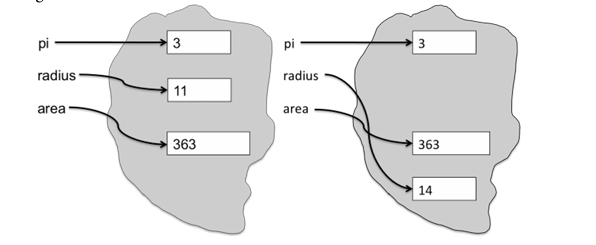
\includegraphics[width=0.7\textwidth]{images/H2.2.png}
    \caption*{Hình 2.2. Ràng buộc biến với đối tượng}
    \label{fig:example}
\end{figure}

Nếu chương trình tiếp tục thực thi lệnh \texttt{radius = 14}, tên radius sẽ được tái liên kết (rebound) với một đối tượng kiểu int khác, như được hiển thị ở bảng bên phải của Hình 2.2. Lưu ý rằng phép gán này không có tác động gì đến giá trị mà area đang liên kết. Biến area vẫn được liên kết với đối tượng được tạo ra từ biểu thức $3 \times (11^2)$.

Trong Python, một biến chỉ đơn thuần là một cái tên, không hơn không kém. Hãy ghi nhớ điều này—nó rất quan trọng. Một câu lệnh gán sẽ liên kết cái tên ở bên trái ký hiệu = với đối tượng được biểu diễn bởi biểu thức ở bên phải ký hiệu =. Cũng hãy ghi nhớ điều này: một đối tượng có thể có một tên, nhiều tên, hoặc không có cái tên nào liên kết với nó cả.

Có lẽ chúng ta không nên nói "một biến chỉ là một cái tên". Bất kể những gì Juliet đã nói$^{11}$, tên gọi thực sự quan trọng. Ngôn ngữ lập trình cho phép chúng ta mô tả các tính toán theo cách mà máy móc có thể thực thi. Điều này không có nghĩa là chỉ có máy tính mới đọc chương trình.

Như bạn sẽ sớm khám phá ra, việc viết các chương trình hoạt động chính xác không phải lúc nào cũng dễ dàng. Các lập trình viên kinh nghiệm sẽ xác nhận rằng họ dành rất nhiều thời gian để đọc các chương trình nhằm cố gắng hiểu tại sao chúng lại hành xử như vậy. Do đó, việc viết chương trình sao cho dễ đọc là điều tối quan trọng. Việc lựa chọn tên biến phù hợp đóng vai trò lớn trong việc tăng cường khả năng đọc hiểu.

Hãy xem xét hai đoạn mã sau:

\begin{verbatim}
# Đoạn mã 1
a = 3.14159    
b = 11.2    
c = a*(b**2)   

# Đoạn mã 2
pi = 3.14159 
diameter = 11.2 
area = pi*(diameter**2)
\end{verbatim}

Đối với Python, chúng không có gì khác biệt. Khi thực thi, chúng sẽ làm cùng một việc. Tuy nhiên, đối với người đọc, chúng lại rất khác nhau. Khi đọc đoạn mã bên trái, không có lý do tiên quyết nào để nghi ngờ có điều gì đó sai sót. Nhưng chỉ cần liếc nhìn đoạn mã bên phải, chúng ta sẽ nảy sinh nghi ngờ ngay: hoặc biến lẽ ra phải tên là radius (bán kính) thay vì diameter (đường kính), hoặc diameter phải được chia cho 2.0 trong phép tính diện tích.

Trong Python, tên biến có thể chứa:
\begin{itemize}
    \item Các chữ cái viết hoa và viết thường
    \item Các chữ số (nhưng không được bắt đầu bằng chữ số)
    \item Ký tự đặc biệt \texttt{\_}
\end{itemize}

Tên biến trong Python có phân biệt chữ hoa chữ thường (ví dụ: Julie và julie là hai tên khác nhau).

Cuối cùng, có một số lượng nhỏ các từ dự phòng (keywords) trong Python đã có sẵn ý nghĩa và không thể dùng làm tên biến. Các từ khóa trong Python 3 bao gồm:

\begin{itemize}
    \item \texttt{and, as, assert, break, class, continue, def, del}
    \item \texttt{elif, else, except, False, finally, for, from, global}
    \item \texttt{if, import, in, is, lambda, nonlocal, None, not}
    \item \texttt{or, pass, raise, return, True, try, while, with, yield}
\end{itemize}

Một cách tốt khác để tăng khả năng đọc hiểu mã nguồn là thêm vào các chú thích (comments). Văn bản đứng sau ký hiệu \texttt{\#} sẽ không được Python thông dịch. Ví dụ:

\begin{verbatim}
side = 1 # Chiều dài cạnh của một hình vuông đơn vị
radius = 1 # Bán kính của một hình tròn đơn vị
# Lấy diện tích hình vuông trừ đi diện tích hình tròn
areaC = pi * radius**2 
areaS = side * side 
difference = areaS - areaC
\end{verbatim}

Python cho phép gán đa luồng (multiple assignment). Câu lệnh:

\begin{verbatim}
x, y = 2, 3
\end{verbatim}

sẽ liên kết x với 2 và y với 3. Tất cả các biểu thức ở phía bên phải của phép gán đều được tính toán trước khi bất kỳ liên kết nào được thay đổi.

Điều này rất tiện lợi vì nó cho phép bạn sử dụng phép gán đa luồng để hoán đổi giá trị liên kết của hai biến. Ví dụ:

\begin{verbatim}
x, y = 2, 3 
x, y = y, x 
print('x =', x) 
print('y =', y)
\end{verbatim}

đoạn mã trên sẽ in ra:

\begin{verbatim}
x = 3 
y = 2
\end{verbatim}

\subsection*{2.1.3 Các trình thông dịch (IDE) của Python}
\addcontentsline{toc}{subsection}{\textcolor{black}{2.1.3 Các trình thông dịch (IDE) của Python}}

\noindent \indent Việc nhập chương trình trực tiếp vào shell là cực kỳ bất tiện. Hầu hết các lập trình viên thích sử dụng một loại trình soạn thảo văn bản nào đó vốn là một phần của Môi trường Phát triển Tích hợp (Integrated Development Environment - IDE).

Một IDE có tên là IDLE được đi kèm sẵn trong gói cài đặt chuẩn của Python. Khi Python trở nên phổ biến hơn, các IDE khác cũng đã xuất hiện. Những IDE mới này thường tích hợp một số thư viện Python phổ biến và cung cấp các tiện ích mà IDLE không có. Anaconda và Canopy là hai trong số những IDE phổ biến nhất hiện nay. Các mã nguồn xuất hiện trong cuốn sách này được tạo và kiểm thử bằng Anaconda.

IDE là các ứng dụng, giống như bất kỳ ứng dụng nào khác trên máy tính của bạn. Hãy khởi động chúng theo cách bạn vẫn làm với các ứng dụng khác, ví dụ như nhấp đúp vào một biểu tượng.

Tất cả các IDE của Python đều cung cấp:
\begin{itemize}
    \item Một trình soạn thảo văn bản với các tính năng:
    \begin{itemize}
        \item Làm nổi bật cú pháp (syntax highlighting)
        \item Tự động hoàn thành mã (auto completion)
        \item Thụt lề thông minh (smart indentation)
    \end{itemize}
    
    \item Một shell có tính năng làm nổi bật cú pháp
    
    \item Một trình gỡ lỗi tích hợp (integrated debugger), thứ mà hiện tại bạn có thể tạm thời bỏ qua
\end{itemize}

Khi IDE khởi động, nó sẽ mở một cửa sổ shell để bạn có thể nhập các lệnh Python. Nó cũng cung cấp cho bạn một menu tệp (File) và một menu chỉnh sửa (Edit), cùng với một số menu khác giúp việc thực hiện các thao tác như in chương trình trở nên thuận tiện hơn.

Menu tệp (File menu) bao gồm các lệnh để:
\begin{itemize}
    \item Tạo một cửa sổ soạn thảo mới để bạn nhập chương trình Python
    \item Mở một tệp chứa chương trình Python hiện có
    \item Lưu nội dung của cửa sổ soạn thảo hiện tại vào một tệp (với phần mở rộng là \texttt{.py})
\end{itemize}

Menu chỉnh sửa (Edit menu) bao gồm các lệnh soạn thảo văn bản tiêu chuẩn:
\begin{itemize}
    \item Các lệnh cơ bản như sao chép (copy), dán (paste) và tìm kiếm (find)
    \item Các lệnh được thiết kế riêng để chỉnh sửa mã Python dễ dàng hơn, chẳng hạn như:
    \begin{itemize}
        \item Thụt lề vùng chọn (indent region)
        \item Chú thích hóa vùng chọn (comment out region)
    \end{itemize}
\end{itemize}

Để biết thêm thông tin về một số IDE phổ biến, hãy truy cập:
\begin{itemize}
    \item \texttt{http://docs.python.org/library/idle.html/}
    \item \texttt{https://store.continuum.io/cshop/anaconda/}
    \item \texttt{https://www.enthought.com/products/canopy/}
\end{itemize}

%=============SEC================
\section*{2.2 Chương trình rẽ nhánh}
\addcontentsline{toc}{section}{\textcolor{black}{2.2 Chương trình rẽ nhánh}}

\noindent \indent Các loại tính toán mà chúng ta đã xem xét cho đến nay được gọi là chương trình tuyến tính (straight-line programs). Chúng thực thi hết câu lệnh này đến câu lệnh khác theo thứ tự xuất hiện và dừng lại khi không còn câu lệnh nào nữa. Những loại tính toán mà chúng ta có thể mô tả bằng chương trình tuyến tính thường không mấy thú vị; thực tế, chúng khá là nhàm chán.

Các chương trình rẽ nhánh (branching programs) thì thú vị hơn nhiều. Câu lệnh rẽ nhánh đơn giản nhất là câu lệnh điều kiện (conditional). Như được trình bày trong phần đóng khung của Hình 2.3, một câu lệnh điều kiện gồm ba phần:

\begin{itemize}
    \item Một phép thử (test): tức là một biểu thức có giá trị tính toán là True (Đúng) hoặc False (Sai)
    
    \item Một khối mã (block of code): sẽ được thực thi nếu phép thử cho kết quả là True
    
    \item Một khối mã tùy chọn (optional block of code): sẽ được thực thi nếu phép thử cho kết quả là False
\end{itemize}

Sau khi một câu lệnh điều kiện được thực thi, việc thực thi chương trình sẽ tiếp tục tại phần mã nằm sau câu lệnh đó.

\begin{figure}[H]
    \centering
    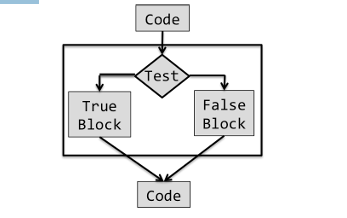
\includegraphics[width=0.6\textwidth]{images/H2.3.png}
    \caption*{Hình 2.3: Lưu đồ cho câu lệnh điều kiện}
    \label{fig:example}
\end{figure}


Trong Python, một câu lệnh điều kiện có dạng:

\begin{verbatim}
if biểu thức Boolean:
    khối mã
else:
    khối mã
\end{verbatim}

hoặc

\begin{verbatim}
if biểu thức Boolean:
    khối mã
\end{verbatim}

Khi mô tả dạng thức của các câu lệnh Python, chúng tôi sử dụng chữ in nghiêng để mô tả các loại mã có thể xuất hiện tại vị trí đó trong chương trình. Ví dụ, biểu thức Boolean chỉ ra rằng bất kỳ biểu thức nào có giá trị True hoặc False đều có thể đứng sau từ khóa \texttt{if}, và khối mã chỉ ra rằng bất kỳ chuỗi câu lệnh Python nào cũng có thể đứng sau \texttt{else:}.

Hãy xem xét chương trình sau đây, nó sẽ in ra "Even" (Chẵn) nếu giá trị của biến x là số chẵn và in "Odd" (Lẻ) trong trường hợp ngược lại:

\begin{verbatim}
if x % 2 == 0:
    print('Even')
else:
    print('Odd')
print('Done with conditional')
\end{verbatim}

Biểu thức \texttt{x \% 2 == 0} sẽ trả về True khi phần dư của x chia cho 2 bằng 0, và trả về False trong các trường hợp còn lại. Hãy nhớ rằng \texttt{==} được dùng để so sánh, vì dấu \texttt{=} đã được dành riêng cho phép gán.

Việc thụt lề (indentation) có ý nghĩa quan trọng về mặt ngữ nghĩa trong Python. Ví dụ, nếu câu lệnh cuối cùng trong đoạn mã trên được thụt lề, nó sẽ trở thành một phần của khối mã liên kết với \texttt{else}, thay vì là khối mã nằm sau câu lệnh điều kiện.

Python khá khác biệt khi sử dụng việc thụt lề theo cách này. Hầu hết các ngôn ngữ lập trình khác sử dụng một số loại ký hiệu đóng ngoặc để phân định các khối mã, ví dụ: C bao bọc các khối mã trong dấu ngoặc nhọn \{ \}. Một ưu điểm của cách tiếp cận trong Python là nó đảm bảo cấu trúc trực quan của chương trình là một sự thể hiện chính xác cấu trúc ngữ nghĩa của chương trình đó. Vì thụt lề có ý nghĩa quan trọng về mặt ngữ nghĩa, nên khái niệm về một ``dòng mã'' là rất quan trọng.

Khi khối đúng (true block) hoặc khối sai (false block) của một câu lệnh điều kiện chứa một câu lệnh điều kiện khác, các câu lệnh điều kiện đó được gọi là lồng nhau (nested). Trong đoạn mã dưới đây, có các câu lệnh điều kiện lồng nhau ở cả hai nhánh của câu lệnh if cấp cao nhất:

\begin{verbatim}
if x % 2 == 0:
    if x % 3 == 0:
        print('Divisible by 2 and 3')
    else:
        print('Divisible by 2 and not by 3')
elif x % 3 == 0:
    print('Divisible by 3 and not by 2')
\end{verbatim}

Từ khóa \texttt{elif} trong đoạn mã trên là viết tắt của ``else if''.

Việc sử dụng một biểu thức Boolean phức hợp trong phép thử của một câu lệnh điều kiện thường rất tiện lợi, ví dụ:

\begin{verbatim}
if x < y and x < z:
    print('x is least')
elif y < z:
    print('y is least')
else:
    print('z is least')
\end{verbatim}

Câu lệnh điều kiện cho phép chúng ta viết các chương trình thú vị hơn chương trình tuyến tính, nhưng lớp các chương trình rẽ nhánh vẫn còn khá hạn chế. Một cách để tư duy về sức mạnh của một lớp chương trình là dựa trên thời gian thực thi của chúng. Giả sử mỗi dòng mã mất một đơn vị thời gian để thực thi. Nếu một chương trình tuyến tính có $n$ dòng mã, nó sẽ mất $n$ đơn vị thời gian để chạy. Vậy còn chương trình rẽ nhánh với $n$ dòng mã thì sao? Nó có thể mất ít hơn $n$ đơn vị thời gian, nhưng không thể nhiều hơn, vì mỗi dòng mã được thực thi tối đa một lần.

Một chương trình mà thời gian chạy tối đa bị giới hạn bởi độ dài của chương trình được gọi là chạy trong thời gian hằng số (constant time). Điều này không có nghĩa là mỗi lần chạy nó đều thực hiện cùng một số bước. Nó có nghĩa là tồn tại một hằng số $k$, sao cho chương trình được đảm bảo không tốn quá $k$ bước để chạy. Điều này ngụ ý rằng thời gian chạy không tăng theo kích thước của dữ liệu đầu vào.

Các chương trình thời gian hằng số khá hạn chế trong những gì chúng có thể làm. Hãy xem xét việc viết một chương trình để kiểm phiếu trong một cuộc bầu cử. Sẽ thật đáng ngạc nhiên nếu ai đó có thể viết một chương trình làm việc này trong một khoảng thời gian độc lập với số lượng phiếu bầu. Thực tế, người ta có thể chứng minh rằng việc đó là bất khả thi. Việc nghiên cứu về độ khó nội tại của các bài toán là chủ đề của độ phức tạp tính toán (computational complexity). Chúng ta sẽ quay lại chủ đề này vài lần trong cuốn sách.

May mắn thay, chúng ta chỉ cần thêm một cấu trúc ngôn ngữ lập trình nữa, đó là vòng lặp (iteration), để có thể viết các chương trình có độ phức tạp tùy ý. Chúng ta sẽ tìm hiểu điều đó trong Mục 2.4.

\noindent \textbf{Bài tập nhỏ (Finger exercise):} Hãy viết một chương trình kiểm tra ba biến—$x$, $y$, và $z$—và in ra số lẻ lớn nhất trong số chúng. Nếu không có số nào là số lẻ, chương trình nên in ra một thông báo tương ứng.

%=============SEC================
\section*{2.3 Chuỗi ký tự và Nhập liệu}
\addcontentsline{toc}{section}{\textcolor{black}{2.3 Chuỗi ký tự và Nhập liệu}}

\noindent \indent Các đối tượng thuộc kiểu \texttt{str} được dùng để biểu diễn các chuỗi ký tự.$^{13}$ Các giá trị trực tiếp (literals) kiểu \texttt{str} có thể được viết bằng dấu ngoặc đơn hoặc ngoặc kép, ví dụ: \texttt{'abc'} hoặc \texttt{"abc"}. Giá trị trực tiếp \texttt{'123'} biểu thị một chuỗi gồm ba ký tự, không phải là con số một trăm hai mươi ba.

Hãy thử nhập các biểu thức sau vào trình thông dịch Python (nhớ rằng \texttt{>>>} là dấu nhắc lệnh, không phải nội dung bạn cần nhập):

\begin{verbatim}
>>> 'a'
>>> 3*4
>>> 3*'a'
>>> 3+4
>>> 'a'+'a'
\end{verbatim}

Toán tử \texttt{+} được gọi là nạp chồng (overloaded): Nó có các ý nghĩa khác nhau tùy thuộc vào kiểu của các đối tượng mà nó được áp dụng. Ví dụ, nó có nghĩa là phép cộng khi áp dụng cho hai con số và là phép nối (concatenation) khi áp dụng cho hai chuỗi. Toán tử \texttt{*} cũng được nạp chồng. Nó mang ý nghĩa như bạn mong đợi khi cả hai toán hạng đều là số. Khi áp dụng cho một số nguyên (\texttt{int}) và một chuỗi (\texttt{str}), nó là một toán tử lặp (repetition) — biểu thức $n*s$, trong đó $n$ là một số nguyên và $s$ là một chuỗi, sẽ tính toán ra một chuỗi gồm $n$ lần lặp lại của $s$. Ví dụ, biểu thức \texttt{2*'John'} có giá trị là \texttt{'JohnJohn'}. Điều này hoàn toàn có logic. Giống như biểu thức toán học $3 \times 2$ tương đương với $2+2+2$, biểu thức \texttt{3*'a'} tương đương với \texttt{'a'+'a'+'a'}.

Bây giờ hãy thử nhập:

\begin{verbatim}
>>> a
>>> 'a'*'a'
\end{verbatim}

Mỗi dòng này đều tạo ra một thông báo lỗi. Dòng đầu tiên tạo ra thông báo:

\begin{verbatim}
NameError: name 'a' is not defined
\end{verbatim}

Vì \texttt{a} không phải là giá trị trực tiếp của bất kỳ kiểu dữ liệu nào, trình thông dịch coi nó như một cái tên (biến). Tuy nhiên, vì cái tên đó chưa được liên kết với bất kỳ đối tượng nào, việc cố gắng sử dụng nó sẽ gây ra lỗi thực thi (runtime error).

Mã \texttt{'a'*'a'} tạo ra thông báo lỗi:

\begin{verbatim}
TypeError: can't multiply sequence by non-int of type 'str'
\end{verbatim}

Việc tồn tại cơ chế kiểm tra kiểu (type checking) là một điều tốt. Nó biến những sai sót vô ý (và đôi khi tinh vi) thành các lỗi làm dừng việc thực thi, thay vì những lỗi khiến chương trình hành xử theo những cách bí ẩn. Việc kiểm tra kiểu trong Python không chặt chẽ như một số ngôn ngữ lập trình khác (ví dụ: Java), nhưng nó tốt hơn trong Python 3 so với Python 2. Ví dụ, khá rõ ràng về ý nghĩa của dấu \texttt{<} khi nó được dùng để so sánh hai chuỗi hoặc hai con số. Nhưng giá trị của \texttt{'4' < 3} nên là gì? Một cách khá tùy tiện, những nhà thiết kế Python 2 đã quyết định nó nên là \texttt{False}, vì tất cả các giá trị số đều nhỏ hơn tất cả các giá trị thuộc kiểu \texttt{str}. Những nhà thiết kế Python 3 và hầu hết các ngôn ngữ hiện đại khác đã quyết định rằng vì những biểu thức như vậy không có ý nghĩa rõ ràng, chúng nên tạo ra một thông báo lỗi.

Chuỗi là một trong số các kiểu tuần tự (sequence types) trong Python. Chúng chia sẻ các thao tác sau với tất cả các kiểu tuần tự khác:

\begin{itemize}
    \item Độ dài của một chuỗi có thể được tìm thấy bằng hàm \texttt{len}. Ví dụ, giá trị của \texttt{len('abc')} là 3.
    
    \item Truy xuất chỉ số (Indexing) có thể được dùng để trích xuất các ký tự riêng lẻ từ một chuỗi. Trong Python, tất cả việc đánh chỉ số đều bắt đầu từ số 0 (zero-based). Ví dụ, nhập \texttt{'abc'[0]} vào trình thông dịch sẽ khiến nó hiển thị chuỗi \texttt{'a'}. Nhập \texttt{'abc'[3]} sẽ tạo ra thông báo lỗi \texttt{IndexError: string index out of range}. Vì Python sử dụng 0 để chỉ phần tử đầu tiên của chuỗi, phần tử cuối cùng của một chuỗi có độ dài bằng 3 được truy cập bằng chỉ số 2. Các số âm được dùng để đánh chỉ số tính từ cuối chuỗi. Ví dụ, giá trị của \texttt{'abc'[-1]} là \texttt{'c'}.
    
    \item Cắt chuỗi (Slicing) được dùng để trích xuất các chuỗi con có độ dài tùy ý. Nếu \texttt{s} là một chuỗi, biểu thức \texttt{s[start:end]} biểu thị chuỗi con của \texttt{s} bắt đầu tại chỉ số \texttt{start} và kết thúc tại chỉ số \texttt{end-1}. Ví dụ, \texttt{'abc'[1:3] == 'bc'}. Tại sao nó lại kết thúc ở chỉ số \texttt{end-1} thay vì \texttt{end}? Để những biểu thức như \texttt{'abc'[0:len('abc')]} có giá trị đúng như mong đợi. Nếu giá trị trước dấu hai chấm bị bỏ trống, nó mặc định là 0. Nếu giá trị sau dấu hai chấm bị bỏ trống, nó mặc định là độ dài của chuỗi. Do đó, biểu thức \texttt{'abc'[:]} có ngữ nghĩa tương đương với biểu thức dài dòng hơn là \texttt{'abc'[0:len('abc')]}.
\end{itemize}

\subsection*{2.3.1 Nhập liệu (Input)}
\addcontentsline{toc}{subsection}{\textcolor{black}{2.3.1 Nhập liệu (Input)}}

\noindent \indent Python 3 có một hàm là \texttt{input}, được dùng để nhận dữ liệu nhập trực tiếp từ người dùng.$^{14}$ Hàm này nhận một chuỗi làm đối số và hiển thị chuỗi đó như một lời nhắc (prompt) trong shell. Sau đó, nó đợi người dùng nhập nội dung và nhấn phím Enter. Dòng dữ liệu mà người dùng đã nhập sẽ được coi là một chuỗi và trở thành giá trị trả về của hàm.

Hãy xem xét đoạn mã sau:

\begin{verbatim}
>>> name = input('Enter your name: ') 
Enter your name: George Washington 
>>> print('Are you really', name, '?') 
Are you really George Washington ? 
>>> print('Are you really ' + name + '?')  
Are you really George Washington?
\end{verbatim}

Lưu ý rằng câu lệnh \texttt{print} đầu tiên đã chèn một khoảng trắng trước dấu \texttt{"?"}. Điều này xảy ra bởi vì khi hàm \texttt{print} nhận nhiều đối số, nó sẽ tự động đặt một khoảng cách giữa các giá trị liên kết với các đối số đó. Câu lệnh \texttt{print} thứ hai sử dụng phép nối chuỗi (concatenation) để tạo ra một chuỗi không chứa khoảng trắng thừa và truyền chuỗi này làm đối số duy nhất cho hàm \texttt{print}.

Bây giờ, hãy xem xét:

\begin{verbatim}
>>> n = input('Enter an int: ') 
Enter an int: 3 
>>> print(type(n))
\end{verbatim}

Lưu ý rằng biến \texttt{n} được liên kết với chuỗi \texttt{'3'} chứ không phải số nguyên 3. Vì vậy, ví dụ, giá trị của biểu thức \texttt{n * 4} sẽ là \texttt{'3333'} thay vì 12. Tin tốt là bất khi nào một chuỗi là một giá trị trực tiếp (literal) hợp lệ của một kiểu dữ liệu nào đó, chúng ta đều có thể áp dụng phép chuyển đổi kiểu.

Chuyển đổi kiểu dữ liệu (còn gọi là ép kiểu - type casts) được sử dụng thường xuyên trong mã nguồn Python. Chúng ta sử dụng tên của một kiểu dữ liệu để chuyển đổi các giá trị sang kiểu đó. Ví dụ, giá trị của biểu thức \texttt{int('3') * 4} là 12. Khi một số thực (\texttt{float}) được chuyển đổi sang một số nguyên (\texttt{int}), con số đó sẽ bị cắt bỏ phần thập phân (chứ không phải làm tròn), ví dụ: giá trị của \texttt{int(3.9)} là số nguyên 3.

\subsection*{2.3.2 Chú giải về Mã hóa ký tự (Character Encoding)}
\addcontentsline{toc}{subsection}{\textcolor{black}{2.3.2 Chú giải về Mã hóa ký tự (Character Encoding)}}

\noindent \indent Trong nhiều năm, hầu hết các ngôn ngữ lập trình đã sử dụng một tiêu chuẩn gọi là ASCII để biểu diễn nội bộ các ký tự. Tiêu chuẩn này bao gồm 128 ký tự, đủ để biểu diễn tập hợp các ký tự thông thường xuất hiện trong văn bản tiếng Anh — nhưng không đủ để bao quát các ký tự và các dấu phụ xuất hiện trong tất cả các ngôn ngữ trên thế giới.

Trong những năm gần đây, đã có sự chuyển dịch sang Unicode. Tiêu chuẩn Unicode là một hệ thống mã hóa ký tự được thiết kế để hỗ trợ việc xử lý kỹ thuật số và hiển thị văn bản viết của tất cả các ngôn ngữ. Tiêu chuẩn này chứa hơn 120.000 ký tự khác nhau — bao quát 129 hệ chữ viết hiện đại và lịch sử cùng nhiều bộ ký hiệu khác nhau.

Tiêu chuẩn Unicode có thể được hiện thực hóa bằng các cách mã hóa ký tự nội bộ khác nhau. Bạn có thể chỉ định cho Python biết nên sử dụng bảng mã nào bằng cách chèn một dòng chú thích theo định dạng:

\begin{verbatim}
# -*- coding: tên_bảng_mã -*-
\end{verbatim}

vào dòng đầu tiên hoặc thứ hai của chương trình. Ví dụ:

\begin{verbatim}
# -*- coding: utf-8 -*-
\end{verbatim}

dòng này chỉ thị cho Python sử dụng UTF-8, bảng mã ký tự được sử dụng thường xuyên nhất cho các trang World Wide Web.$^{15}$ Nếu bạn không có dòng chú thích như vậy trong chương trình, hầu hết các bản thực thi Python sẽ mặc định sử dụng UTF-8.

Khi sử dụng UTF-8, nếu trình soạn thảo văn bản cho phép, bạn có thể nhập trực tiếp các đoạn mã như:

\begin{verbatim}
print('Mluvíš anglicky?')
\end{verbatim}

kết quả sẽ in ra:

\begin{verbatim}
Mluvíš anglicky?
\end{verbatim}

Bạn có thể thắc mắc làm thế nào tôi có thể gõ được chuỗi \texttt{'Mluvíš anglicky?'}. Thực tế là tôi không gõ. Bởi vì hầu hết World Wide Web đều sử dụng UTF-8, tôi có thể sao chép chuỗi đó từ một trang web và dán trực tiếp vào chương trình của mình.

%=============SEC================
\section*{2.4 Vòng lặp}
\addcontentsline{toc}{section}{\textcolor{black}{2.4 Vòng lặp}}

\noindent \indent Chúng ta đã kết thúc Mục 2.2 với nhận định rằng hầu hết các tác vụ tính toán không thể hoàn thành chỉ bằng các chương trình rẽ nhánh. Hãy thử tưởng tượng việc viết một chương trình yêu cầu người dùng nhập số lần họ muốn in chữ cái ``X'', sau đó in ra một chuỗi với số lượng chữ X tương ứng. Chúng ta có thể nghĩ đến việc viết như sau:

\begin{verbatim}
numXs = int(input('How many times should I print the letter X? '))
toPrint = ''
if numXs == 1:
    toPrint = 'X'
elif numXs == 2:
    toPrint = 'XX'
elif numXs == 3:
    toPrint = 'XXX'
# ...
print(toPrint)
\end{verbatim}

Nhưng sẽ nhanh chóng nhận thấy rằng chúng ta cần số lượng câu lệnh điều kiện tương đương với số lượng các số nguyên dương — và thực tế là có vô số số nguyên dương. Cái chúng ta thực sự cần là một chương trình có dạng:

\begin{verbatim}
numXs = int(input('How many times should I print the letter X? '))
toPrint = ''
# nối X vào toPrint numXs lần
print(toPrint)
\end{verbatim}

Khi muốn một chương trình thực hiện cùng một việc nhiều lần, chúng ta có thể sử dụng vòng lặp (iteration hay looping). Cơ chế lặp tổng quát được thể hiện trong phần đóng khung của Hình 2.4. Giống như câu lệnh điều kiện, nó bắt đầu bằng một phép thử. Nếu phép thử trả về True, chương trình thực thi thân vòng lặp (loop body) một lần, rồi quay lại đánh giá lại phép thử. Quá trình này lặp lại cho đến khi phép thử trả về False, sau đó quyền điều khiển được chuyển đến đoạn mã nằm sau câu lệnh lặp.

\begin{figure}[H]
    \centering
    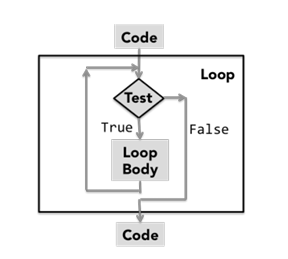
\includegraphics[width=0.6\textwidth]{images/H2.4.png}
    \caption*{Hình 2.4: Lưu đồ cho vòng lặp}
    \label{fig:example}
\end{figure}

Chúng ta có thể viết loại vòng lặp được mô tả trong Hình 2.4 bằng câu lệnh \texttt{while}. Hãy xem ví dụ sau:

\begin{verbatim}
# Tính bình phương một số nguyên bằng phương pháp cộng lặp
x = 3
ans = 0
itersLeft = x
while (itersLeft != 0):
    ans = ans + x
    itersLeft = itersLeft - 1
print(str(x) + '*' + str(x) + ' = ' + str(ans))
\end{verbatim}

Mã nguồn bắt đầu bằng cách liên kết biến $x$ với số nguyên 3. Sau đó, nó thực hiện bình phương $x$ bằng cách cộng lặp lại. Bảng trong Hình 2.5 cho thấy giá trị gắn với mỗi biến mỗi khi chạm đến phép thử ở đầu vòng lặp. Chúng tôi xây dựng bảng này bằng cách mô phỏng thủ công (hand-simulating) đoạn mã, tức là đóng vai một trình thông dịch Python và thực thi chương trình bằng bút và giấy. Sử dụng bút và giấy nghe có vẻ cổ điển, nhưng đó là một cách tuyệt vời để hiểu cách một chương trình vận hành.

\begin{table}[H]
\centering
\caption*{Hình 2.5: Mô phỏng thủ công một chương trình nhỏ}
\label{tab:simulation}
\begin{tabular}{|c|c|c|c|}
\hline
\textbf{Lần thử (Test \#)} & \textbf{x} & \textbf{ans} & \textbf{itersLeft} \\
\hline
1 & 3 & 0 & 3 \\
\hline
2 & 3 & 3 & 2 \\
\hline
3 & 3 & 6 & 1 \\
\hline
4 & 3 & 9 & 0 \\
\hline
\end{tabular}
\end{table}

Lần thứ tư chạm đến phép thử, nó trả về False và luồng điều khiển chuyển đến câu lệnh \texttt{print} nằm sau vòng lặp. Với những giá trị nào của $x$ thì chương trình này sẽ kết thúc? Có ba trường hợp cần xem xét: $x = 0, x > 0,$ và $x < 0$.

\begin{itemize}
    \item Nếu $x = 0$: Giá trị ban đầu của \texttt{itersLeft} cũng sẽ là 0, và thân vòng lặp sẽ không bao giờ được thực thi.
    
    \item Nếu $x > 0$: Giá trị ban đầu của \texttt{itersLeft} sẽ lớn hơn 0, và thân vòng lặp sẽ được thực thi ít nhất một lần. Mỗi lần thực thi thân vòng lặp, giá trị của \texttt{itersLeft} giảm đi đúng 1 đơn vị. Điều này có nghĩa là nếu \texttt{itersLeft} bắt đầu lớn hơn 0, sau một số lần lặp hữu hạn, \texttt{itersLeft} sẽ bằng 0. Tại thời điểm đó, phép thử vòng lặp trả về False và quyền điều khiển chuyển đến mã sau câu lệnh \texttt{while}.
    
    \item Nếu $x < 0$: Một điều rất tệ sẽ xảy ra. Quyền điều khiển sẽ đi vào vòng lặp, và mỗi lần lặp lại khiến \texttt{itersLeft} càng xa số 0 thay vì lại gần nó hơn. Chương trình sẽ tiếp tục thực hiện vòng lặp mãi mãi (vòng lặp vô hạn). Làm thế nào để khắc phục lỗi này? Việc khởi tạo \texttt{itersLeft} bằng giá trị tuyệt đối của $x$ (\texttt{abs(x)}) gần như giải quyết được vấn đề. Vòng lặp sẽ kết thúc, nhưng nó sẽ in ra một giá trị âm. Nếu câu lệnh gán bên trong vòng lặp cũng được đổi thành \texttt{ans = ans + abs(x)}, mã nguồn sẽ hoạt động chính xác.
\end{itemize}

\noindent \textbf{Bài tập nhỏ (Finger exercise):} Hãy thay thế phần chú thích trong đoạn mã sau bằng một vòng lặp \texttt{while}.

\begin{verbatim}
numXs = int(input('How many times should I print the letter X? '))
toPrint = ''
# nối X vào toPrint numXs lần
print(toPrint)
\end{verbatim}

Đôi khi việc thoát khỏi vòng lặp mà không cần kiểm tra điều kiện lặp là rất tiện lợi. Việc thực thi câu lệnh \texttt{break} sẽ chấm dứt vòng lặp chứa nó và chuyển quyền điều khiển đến đoạn mã ngay sau vòng lặp đó. Ví dụ:

\begin{verbatim}
# Tìm một số nguyên dương chia hết cho cả 11 và 12
x = 1
while True:
    if x%11 == 0 and x%12 == 0:
        break
    x = x + 1
print(x, 'is divisible by 11 and 12')
\end{verbatim}

Kết quả in ra: \texttt{132 is divisible by 11 and 12}. Nếu một câu lệnh \texttt{break} được thực thi bên trong một vòng lặp lồng nhau (vòng lặp nằm trong vòng lặp khác), lệnh \texttt{break} sẽ chỉ chấm dứt vòng lặp bên trong cùng chứa nó.

Đến đây, chúng ta đã bao quát hầu hết mọi thứ về Python cần thiết để bắt đầu viết các chương trình thú vị xử lý số và chuỗi. Trong chương tiếp theo, chúng ta sẽ tạm nghỉ việc học Python để sử dụng những gì đã biết giải quyết một số bài toán đơn giản.

\noindent \textbf{Bài tập nhỏ (Finger exercise):} Viết một chương trình yêu cầu người dùng nhập vào 10 số nguyên, sau đó in ra số lẻ lớn nhất trong số các số đã nhập. Nếu không có số lẻ nào được nhập, chương trình nên in ra một thông báo tương ứng.